% -----------------------------*- LaTeX -*------------------------------
\documentclass[UTF8]{report}
% ------------------------------------------------------------------------
% Packages
% ------------------------------------------------------------------------
\usepackage{ctex}
\usepackage[body={7in, 9in},left=1in,right=1in]{geometry}
\usepackage{amsmath,amsfonts,amssymb,bm,amsthm}%数学宏包、数学字体、数学符号、支持 \mathscr{} 字体、支持粗斜体 \bm{}、数学定理
\usepackage{graphicx}%支持 \includegraphics{} 插图
\usepackage{subfigure}%插入子图
\usepackage{nicefrac}
\usepackage{mathrsfs}
\usepackage{caption}
\usepackage{algorithm,algorithmicx}
\usepackage[noend]{algpseudocode}
\usepackage{fancyhdr}
\usepackage{adjustbox}
\usepackage{esint}%支持多种积分算子
\usepackage{mathtools}%数学宏包的重要补充
\usepackage{upgreek}%数学环境的直立希腊字母
\usepackage{enumitem}%自定义列表环境
\usepackage{color}%支持颜色改变
\usepackage{extarrows}%任意长度的箭头
\usepackage{tikz,xcolor}%画图、画 Feynman 图
\usepackage{breqn}
\usepackage{fontsize}
\usepackage[framemethod=TikZ]{mdframed}
\usepackage{fontspec}
\usepackage{bigstrut,multirow,rotating}%Excel表格自动导入latex
\usepackage{booktabs}
\usepackage{scribe}
% ------------------------------------------------------------------------
% Macros
% ------------------------------------------------------------------------
%~~~~~~~~~~~~~~~
% Utility latin
%~~~~~~~~~~~~~~~
\newcommand{\ie}{\textit{i.e.}}
\newcommand{\eg}{\textit{e.g.}}
%~~~~~~~~~~~~~~~
% Environment shortcuts
%~~~~~~~~~~~~~~~
\newcommand{\balign}[1]{\ealign{\begin{align}#1\end{align}}}
\newcommand{\baligns}[1]{\ealigns{\begin{align*}#1\end{align*}}}
\newcommand{\bitemize}[1]{\eitemize{\begin{itemize}#1\end{itemize}}}
\newcommand{\benumerate}[1]{\eenumerate{\begin{enumerate}#1\end{enumerate}}}
%~~~~~~~~~~~~~~~
% Text with quads around it
%~~~~~~~~~~~~~~~
\newcommand{\qtext}[1]{\quad\text{#1}\quad}
%~~~~~~~~~~~~~~~
% Shorthand for math formatting
%~~~~~~~~~~~~~~~
\newcommand{\mbb}[1]{\mathbb{#1}}
\newcommand{\mbi}[1]{\boldsymbol{#1}} % Bold and italic (math bold italic)
\newcommand{\mbf}[1]{\mathbf{#1}}
\newcommand{\mc}[1]{\mathcal{#1}}
\newcommand{\mrm}[1]{\mathrm{#1}}
\newcommand{\tbf}[1]{\textbf{#1}}
\newcommand{\tsc}[1]{\textsc{#1}}
%\def\<{{\langle}}
%\def\>{{\rangle}}
\newcommand{\sT}{\sf T}
\newcommand{\grad}{\nabla}
\newcommand{\Proj}{\Pi}
%~~~~~~~~~~~~~~~
% Common sets 定义数集符号
%~~~~~~~~~~~~~~~
\newcommand{\R}{\mathbb{R}}
\newcommand{\Z}{\mathbb{Z}}
\newcommand{\Q}{\mathbb{Q}}
\newcommand{\N}{\mathbb{N}}
\newcommand{\C}{\mathbb{C}}
\newcommand{\reals}{\mathbb{R}} % Real number symbol
\newcommand{\integers}{\mathbb{Z}} % Integer symbol
\newcommand{\rationals}{\mathbb{Q}} % Rational numbers
\newcommand{\naturals}{\mathbb{N}} % Natural numbers
\newcommand{\complex}{\mathbb{C}} % Complex numbers
%~~~~~~~~~~~~~~~
% Common functions
%~~~~~~~~~~~~~~~
\renewcommand{\exp}[1]{\operatorname{exp}\left(#1\right)} % Exponential
\newcommand{\indic}[1]{\mbb{I}\left(#1\right)} % Indicator function
\newcommand{\indicsub}[2]{\mbb{I}_{#2}\left(#1\right)} % Indicator function
\newcommand{\argmax}{\mathop\mathrm{arg\, max}} % Defining math symbols
\newcommand{\argmin}{\mathop\mathrm{arg\, min}}
\renewcommand{\arccos}{\mathop\mathrm{arccos}}
\newcommand{\dom}{\mathop\mathrm{dom}} % Domain
\newcommand{\range}{\mathop\mathrm{range}} % Range
\newcommand{\diag}{\mathop\mathrm{diag}}
\newcommand{\tr}{\mathop\mathrm{tr}}
\newcommand{\abs}{\mathop\mathrm{abs}}
\newcommand{\card}{\mathop\mathrm{card}}
\newcommand{\sign}{\mathop\mathrm{sign}}
\newcommand{\prox}{\mathrm{prox}} % prox
\newcommand{\rank}[1]{\mathrm{rank}(#1)}
\newcommand{\supp}[1]{\mathrm{supp}(#1)}
\newcommand{\norm}[1]{\lVert#1\rVert}
%~~~~~~~~~~~~~~~
% Common probability symbols
%~~~~~~~~~~~~~~~
\newcommand{\family}{\mathcal{P}} % probability family / statistical model
\newcommand{\iid}{\stackrel{\mathrm{iid}}{\sim}}
\newcommand{\ind}{\stackrel{\mathrm{ind}}{\sim}}
\newcommand{\E}{\mathbb{E}} % Expectation symbol
\newcommand{\Earg}[1]{\E\left[#1\right]}
\newcommand{\Esubarg}[2]{\E_{#1}\left[#2\right]}
\renewcommand{\P}{\mathbb{P}} % Probability symbol
\newcommand{\Parg}[1]{\P\left(#1\right)}
\newcommand{\Psubarg}[2]{\P_{#1}\left[#2\right]}
%\newcommand{\Cov}{\mrm{Cov}} % Covariance symbol
%\newcommand{\Covarg}[1]{\Cov\left[#1\right]}
%\newcommand{\Covsubarg}[2]{\Cov_{#1}\left[#2\right]}
%\newcommand{\model}{\mathcal{P}} % probability family / statistical model
%~~~~~~~~~~~~~~~
% Distributions
%~~~~~~~~~~~~~~~
%\newcommand{\Gsn}{\mathcal{N}}
%\newcommand{\Ber}{\textnormal{Ber}}
%\newcommand{\Bin}{\textnormal{Bin}}
%\newcommand{\Unif}{\textnormal{Unif}}
%\newcommand{\Mult}{\textnormal{Mult}}
%\newcommand{\NegMult}{\textnormal{NegMult}}
%\newcommand{\Dir}{\textnormal{Dir}}
%\newcommand{\Bet}{\textnormal{Beta}}
%\newcommand{\Gam}{\textnormal{Gamma}}
%\newcommand{\Poi}{\textnormal{Poi}}
%\newcommand{\HypGeo}{\textnormal{HypGeo}}
%\newcommand{\GEM}{\textnormal{GEM}}
%\newcommand{\BP}{\textnormal{BP}}
%\newcommand{\DP}{\textnormal{DP}}
%\newcommand{\BeP}{\textnormal{BeP}}
%\newcommand{\Exp}{\textnormal{Exp}}
%~~~~~~~~~~~~~~~
% Theorem-like environments
%~~~~~~~~~~~~~~~
%\theoremstyle{definition}
%\newtheorem{definition}{Definition}
%\newtheorem{example}{Example}
%\newtheorem{problem}{Problem}
%\newtheorem{lemma}{Lemma}
%~~~~~~~~~~~~~~~
% 组合数学的模板和作业里用到的一些宏包和自定义命令
%~~~~~~~~~~~~~~~
\renewcommand{\emph}[1]{\begin{kaishu}#1\end{kaishu}}
\newcommand{\falfac}[1]{^{\underline{#1}}}
\newcommand{\binomfrac}[2]{\frac{#1^{\underline{#2}}}{#2!}}
\newcommand{\ceil}[1]{\left\lceil #1 \right\rceil}
\newcommand{\floor}[1]{\left\lfloor #1 \right\rfloor}
\newcommand{\suminfty}[2]{\sum_{#1=#2}^{\infty}}
\newcommand{\suminftyk}[0]{\sum_{k=0}^{\infty}}
\newcommand{\sumint}[3]{\sum_{#1=#2}^{#3}}
\newcommand{\sumintk}[2]{\sum_{k=#1}^{#2}}
\newcommand{\suminti}[2]{\sum_{i=#1}^{#2}}
%~~~~~~~~~~~~~~~
% 定义新命令
%~~~~~~~~~~~~~~~
\newcommand*{\unit}[1]{\mathop{}\!\mathrm{#1}}
\newcommand*{\dif}{\mathop{}\!\mathrm{d}}%微分算子 d
\newcommand*{\pdif}{\mathop{}\!\partial}%偏微分算子
\newcommand*{\cdif}{\mathop{}\!\nabla}%协变导数、nabla 算子
\newcommand*{\laplace}{\mathop{}\!\Delta}%laplace 算子
\newcommand*{\deriv}[2]{\frac{\mathrm{d} #1}{\mathrm{d} {#2}}}
\newcommand*{\derivh}[3]{\frac{\mathrm{d}^{#1} #2}{\mathrm{d} {#3^{#1}}}}
\newcommand*{\pderiv}[2]{\frac{\partial #1}{\partial {#2}}}
\newcommand*{\pderivh}[3]{\frac{\partial^{#1} #2}{\partial {#3^{#1}}}}
\newcommand*{\dderiv}[2]{\dfrac{\mathrm{d} #1}{\mathrm{d} {#2}}}
\newcommand*{\dderivh}[3]{\dfrac{\mathrm{d}^{#1} #2}{\mathrm{d} {#3^{#1}}}}
\newcommand*{\dpderiv}[2]{\dfrac{\partial #1}{\partial {#2}}}
\newcommand*{\dpderivh}[3]{\dfrac{\partial^{#1} #2}{\partial {#3^{#1}}}}
\newcommand{\me}[1]{\mathrm{e}^{#1}}%e 指数
\newcommand{\mi}{\mathrm{i}}%虚数单位
%\newcommand{\mc}{\mathrm{c}}%光速 定义与mathcal冲突
\newcommand{\red}[1]{\textcolor{red}{#1}}
\newcommand{\blue}[1]{\textcolor{blue}{#1}}
%\newcommand{\Rome}[1]{\setcounter{rome}{#1}\Roman{rome}}
%~~~~~~~~~~~~~~~
% 公式环境中箭头符号的简写
%~~~~~~~~~~~~~~~
\newcommand{\ra}{\rightarrow}
\newcommand{\Ra}{\Rightarrow}
\newcommand{\la}{\leftarrow}
\newcommand{\La}{\Leftarrow}
\newcommand{\lra}{\leftrightarrow}
\newcommand{\Lra}{\Leftrightarrow}
\newcommand{\lgla}{\longleftarrow}
\newcommand{\Lgla}{\Longleftarrow}
\newcommand{\lgra}{\longrightarrow}
\newcommand{\Lgra}{\Longrightarrow}
\newcommand{\lglra}{\longleftrightarrow}
\newcommand{\Lglra}{\Longleftrightarrow}
%~~~~~~~~~~~~~~~
% 一些数学的环境设置
%~~~~~~~~~~~~~~~
%\newcounter{counter_exm}\setcounter{counter_exm}{1}
%\newcounter{counter_prb}\setcounter{counter_prb}{1}
%\newcounter{counter_thm}\setcounter{counter_thm}{1}
%\newcounter{counter_lma}\setcounter{counter_lma}{1}
%\newcounter{counter_dft}\setcounter{counter_dft}{1}
%\newcounter{counter_clm}\setcounter{counter_clm}{1}
%\newcounter{counter_cly}\setcounter{counter_cly}{1}
%\newtheorem{theorem}{{\hskip 1.7em \bf 定理}}
%\newtheorem{lemma}[theorem]{\hskip 1.7em 引理}
%\newtheorem{proposition}[theorem]{Proposition}
%\newtheorem{claim}[theorem]{\hskip 1.7em 命题}
%\newtheorem{corollary}[theorem]{\hskip 1.7em 推论}
%\newtheorem{definition}[theorem]{\hskip 1.7em 定义}
\newcommand{\problem}[1]{{\setlength{\parskip}{10pt}\noindent \bf{#1}}}
\newenvironment{solution}{{\noindent\hskip 2em \bf 解 \quad}}{}
\renewenvironment{proof}{{\setlength{\parskip}{7pt}\noindent\hskip 2em \bf 证明 \quad}}{\hfill$\qed$\par}
%\newenvironment{example}{{\noindent\hskip 2em \bf 例 \arabic{counter_exm}\quad}}{\addtocounter{counter_exm}{1}\par}
%\newenvironment{concept}[1]{{\bf #1\quad} \begin{kaishu}} {\end{kaishu}\par}

% ----------------------------------------------------------------------
% Header information
% ------------------------------------------------------------------------

\begin{document}

\course{B0911005Y-01} 			%optional
\coursetitle{Introduction to Theory of Computation}	%optional
\semester{2023 Spring}		%optional
\lecturer{Mingji Xia}	%optional
\scribe{吉骏雄}		%required
\lecturenumber{3}			%required (must be a number)
\lecturedate{March 31}	%required (omit year)

\maketitle

% ----------------------------------------------------------------------
% Body of the document
% ------------------------------------------------------------------------


\textbf{第3.1次作业: 3.1(d), 3.2(d).}
\textbf{勘误: 图3-4, $q_5$状态上的$x\ra R$改为$x\ra L$}


\problem{3.1} 此练习与图灵机$M_2$有关, 例3.4给出了它的描述及状态图. 在下列每个输入串上, 给出$M_2$所进入的格局序列. 例3.4中$M_2$如下:

描述图灵机$M_2$, 它判定的语言是所有由$0$组成、长度为$2$的方幂的字符串, 即$A = \{ 0^{2^n} \mid n\geq 0\}$.

下面给出$M_2 = (Q, \Sigma, \Gamma, \delta, q_1, q_{\text{accept}}, q_{\text{reject}})$的形式化描述:
\begin{itemize}
    \item $Q = \{q_1, q_2, q_3, q_4, q_5, q_{\text{accept}}, q_{\text{reject}}\}$
    \item $\Sigma = \{0\}$
    \item $\Gamma = \{0, x, \sqcup\}$
    \item 状态转移如图\ref{fig:3_1}
\end{itemize}
\begin{figure}[!htbp]
    \centering
    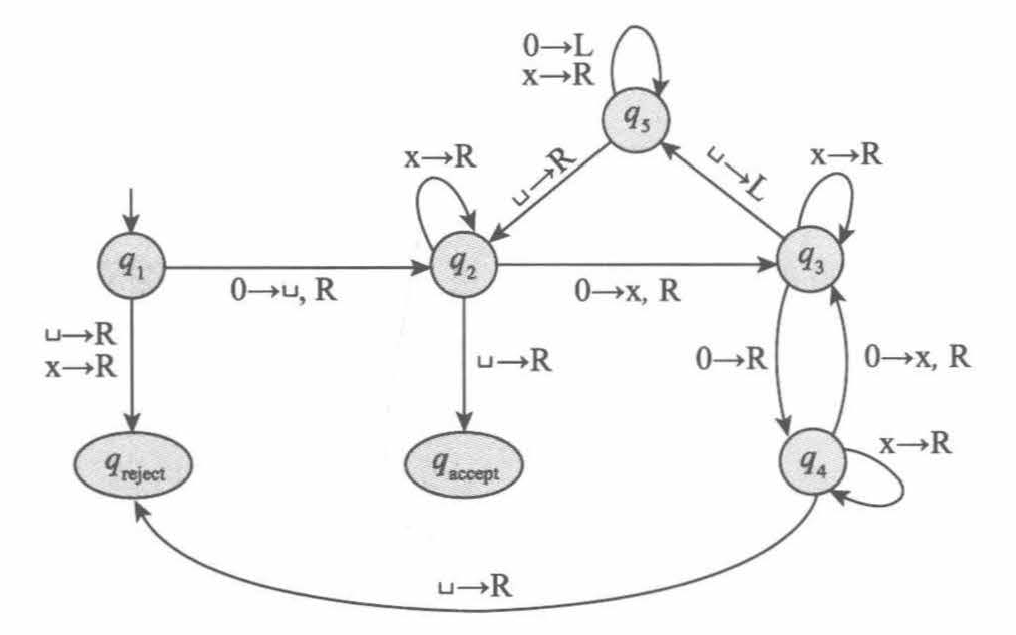
\includegraphics[width=8cm]{image/3.1.png}
    \caption{例3.4 图灵机$M_2$的状态图 ($q_5$上状态有误)}
    \label{fig:3_1}
\end{figure}

\problem{(d)} $000000$ (注: 一共$6$个$0$)

\begin{align*}
    &q_1 000000,\ \sqcup q_200000,\ \sqcup xq_3 0000,\ \sqcup x0 q_4 000,\ \sqcup x0x q_3 00,\ \sqcup x0x0 q_4 0,\ \sqcup x0x0x q_3,\\
    &\sqcup x0x0 q_5 x,\ \sqcup x0x q_5 0x,\ \sqcup x0 q_5 x0x,\ \sqcup x q_5 0x0x,\ \sqcup q_5 x0x0x,\ q_5 \sqcup x0x0x,\ \sqcup q_2 x0x0x\\
    &\sqcup x q_2 0x0x,\ \sqcup xx q_3 x0x,\ \sqcup xxx q_3 0x,\ \sqcup xxx0 q_4 x,\ \sqcup xxx0x q_4,\ \sqcup xxx0x q_{\text{reject}}
\end{align*}


\problem{3.2} 此练习与图灵机$M_1$有关, 例3.5给出了它的描述及状态图. 在下列每个输入串上, 给出$M_1$所进入的格局序列. 例3.5中$M_1$如下:

$M_1 = (Q, \Sigma, \Gamma, \delta, q_1, q_{\text{accept}}, q_{\text{reject}})$, 它判定的语言是 $B = \{ w \# w \mid w \in \{0,1\}^* \}$
状态转移如图\ref{fig:3_2}
\begin{figure}[!htbp]
    \centering
    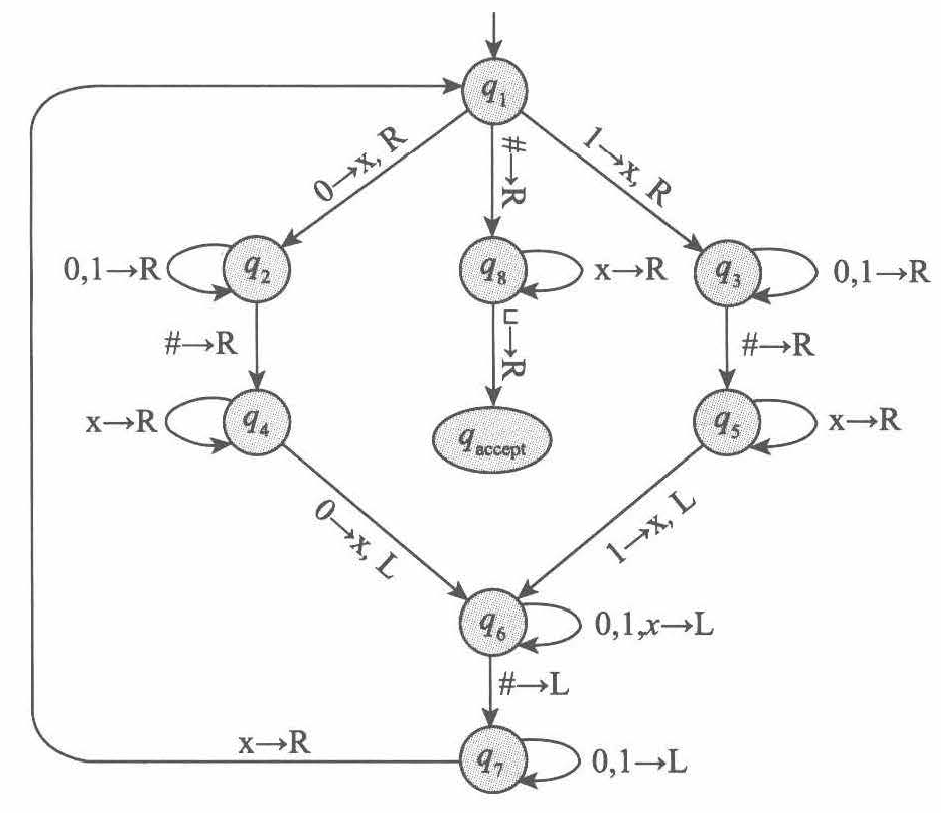
\includegraphics[width=8cm]{image/3.2.png}
    \caption{例3.5 图灵机$M_1$的状态图}
    \label{fig:3_2}
\end{figure}

\problem{(d)} $10\#11$

\begin{align*}
    & q_1 10\#11,\ x q_3 0\#11,\ x0 q_3 \#11,\ x0\# q_5 11,\ x0 q_6 \#x1,\ x q_7 0\#x1,\\
    & q_7 x0\#x1,\ x q_1 0\#x1,\ xx q_2 \#x1,\ xx\# q_4 x1,\ xx\#x q_4 1,\ xx\#x q_{\text{reject}} 1
\end{align*}



\textbf{第3.2次作业:3.9. 补充题 (见题目). 选做题:3.22}

\problem{3.9} 设$A $是仅含一个串$s $的语言, 其中:
\[
    s= \begin{cases*}
        $0$ & 如果火星上没有任何生命 \\
        $1$ & 如果火星上发现生命
    \end{cases*}
\]
$A $是可判定的吗?为什么?在本题中, 假设 ``火星上是否有生命'' 这一问题的答案只有 ``有'' 或 ``没有'' 两种. 

\begin{solution}
    是可判定的. 因为$A$只有两种可能: $\{0\}$ 或者 $\{1\}$. 这两个都是有限的语言, 因而都是图灵可判定的, 很容易能给出两个图灵机的构造, 分别识别这两种语言, 如图\ref{fig:3_9}. 虽然我们并不知道到底哪一个能识别$A$, 但是一定有一个可以.
    \begin{figure}[!htbp]
        \centering
        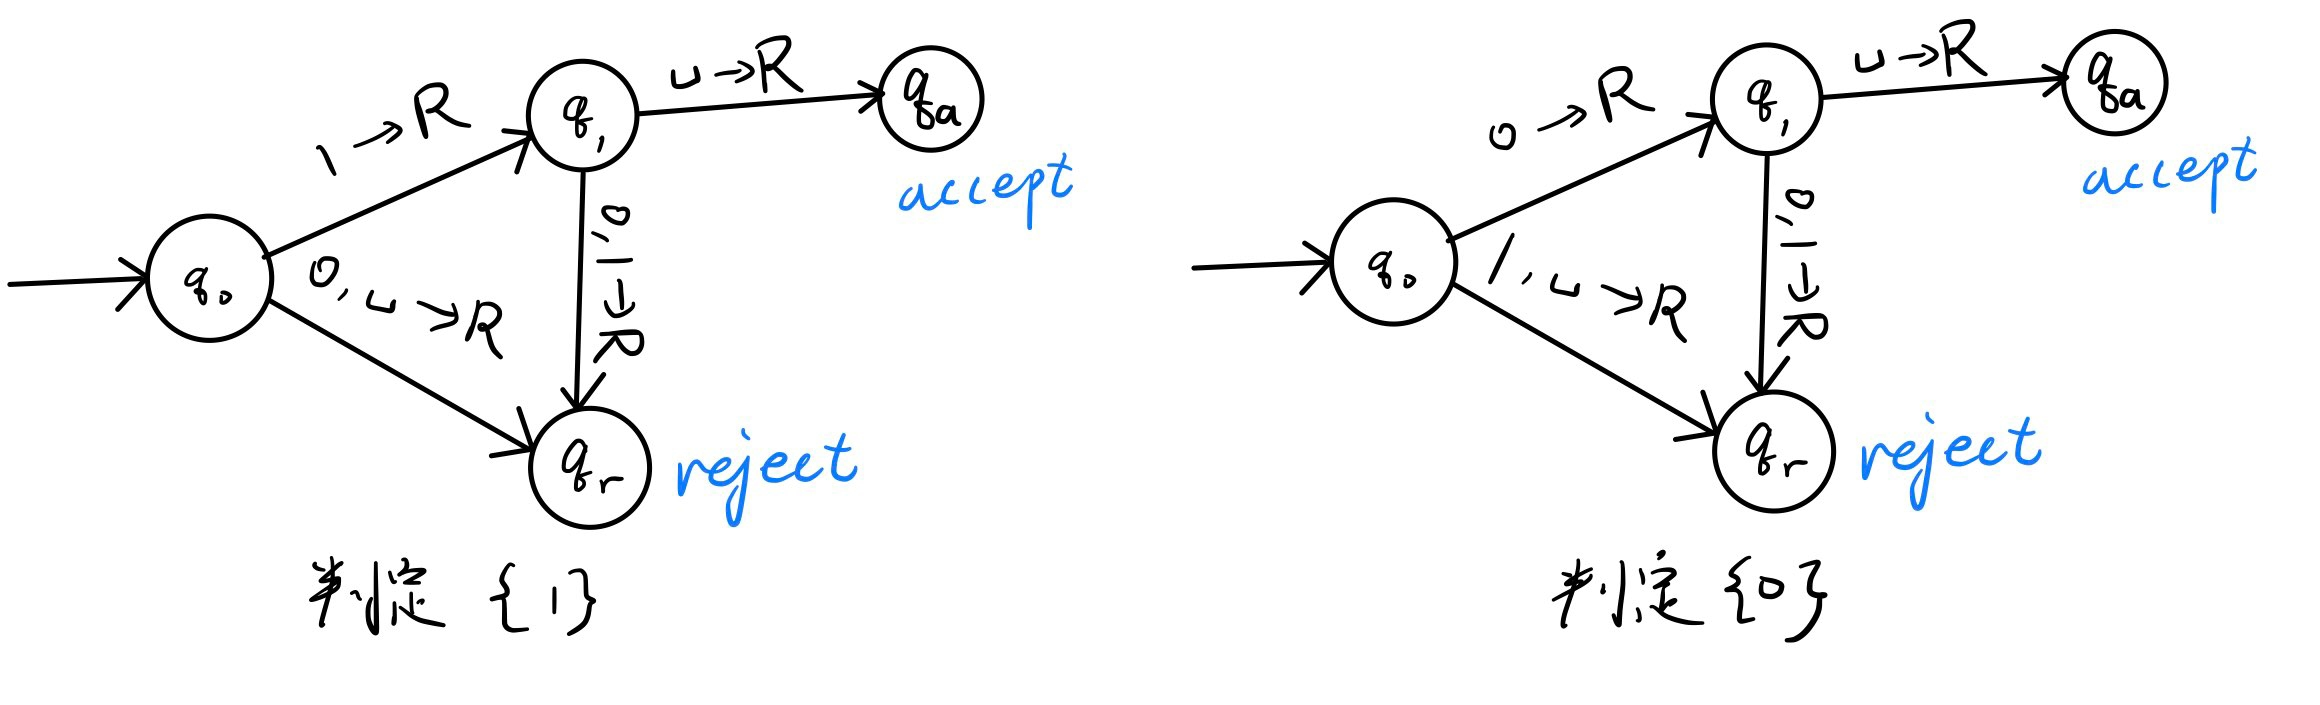
\includegraphics[width=10cm]{image/3.9.png}
        \caption{3.9}
        \label{fig:3_9}
    \end{figure}
\end{solution}

\problem{补充题:} 对于字母表$\{0,1\}$上的语言$\{\omega \mid \omega \text{ 所包含的 }0\text{ 的个数是 }1\text{ 的个数的两倍}\}$:
\begin{enumerate}
    \item 给出识别它的下推自动机的状态图
    \item 以高层次描述给出判定它的图灵机
    \item 基于2, 画出判定它的图灵机的状态图
\end{enumerate}

\begin{solution}
    \begin{enumerate}
        \item 如图\ref{fig:3_补充题1}.

        \begin{figure}[!htbp]
            \centering
            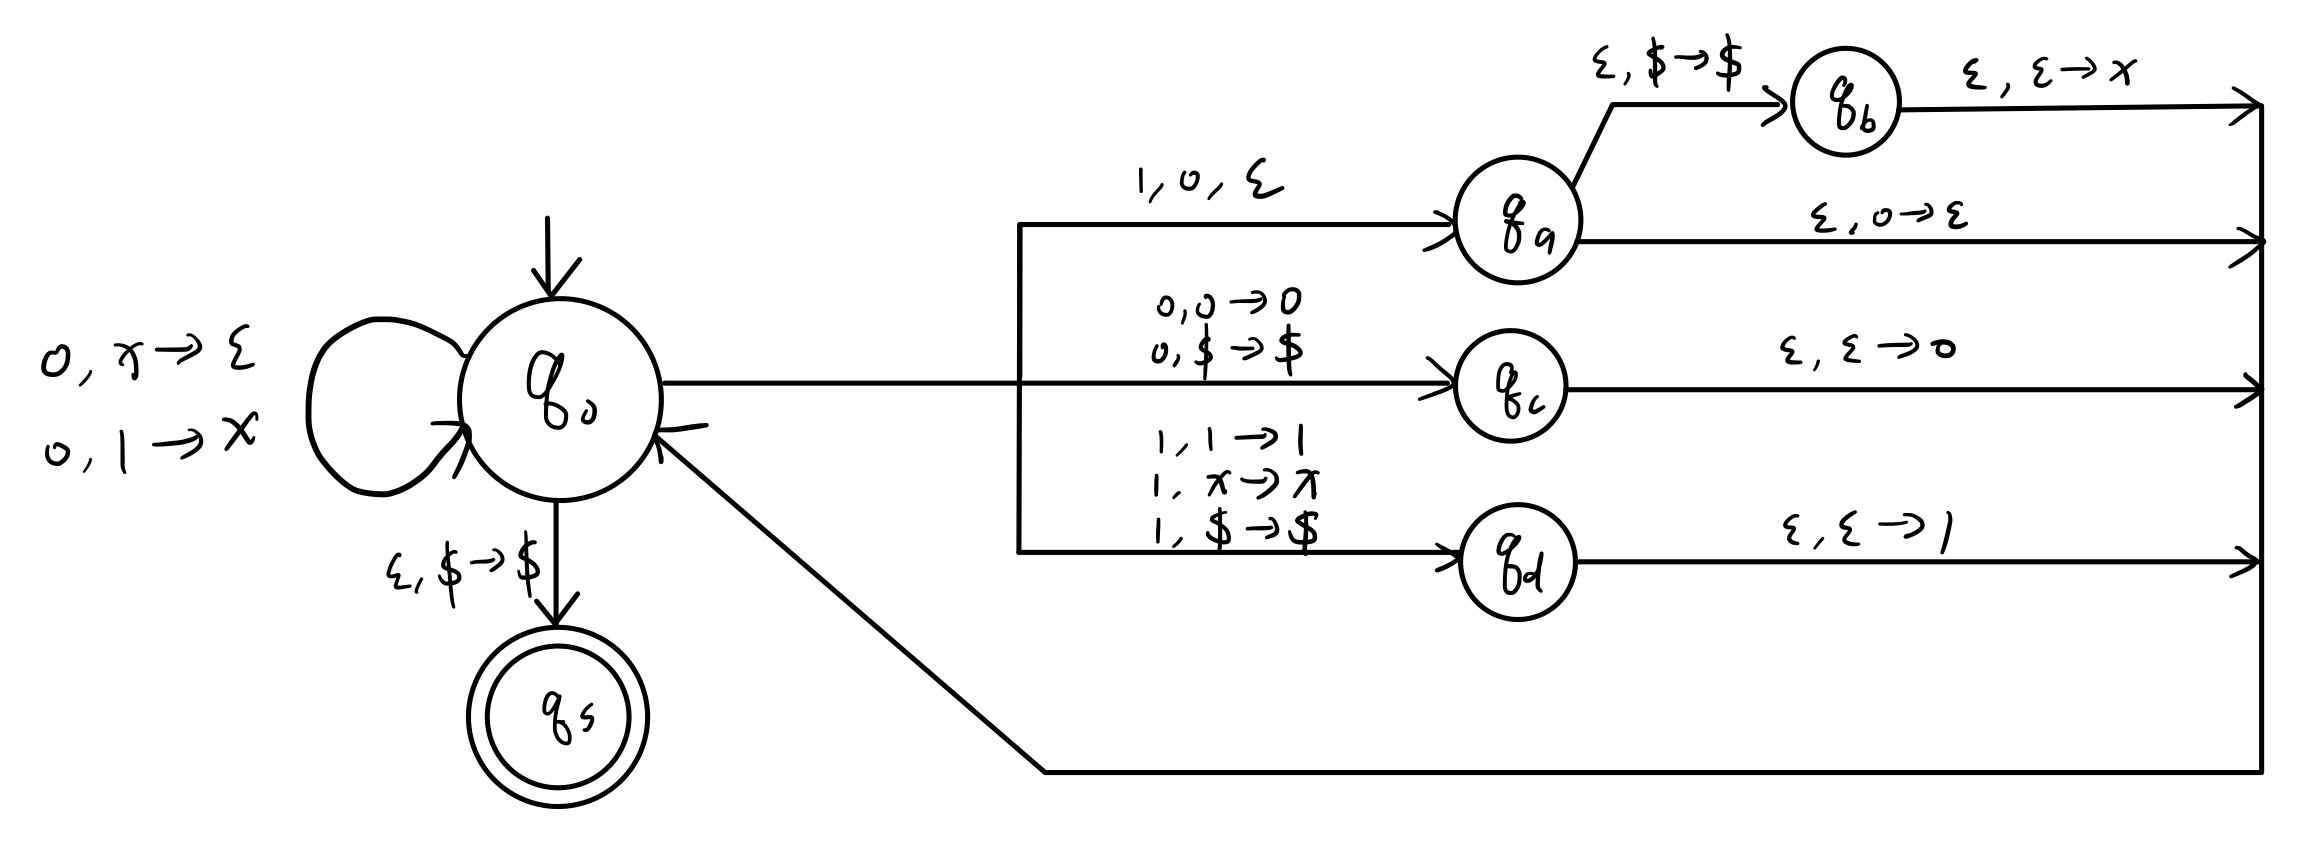
\includegraphics[width=10cm]{image/3.补充题1.png}
            \caption{3.补充题1}
            \label{fig:3_补充题1}
        \end{figure}

        \item 从字符串的左侧向右读. 每当读到一个0时, 消去这个0, 并且向右走, 消去最近的一个0和一个1再返回; 每当读到一个1时, 消去这个1, 并且向右走, 消去最近的两个0再返回; 读到x, 直接将之改为空, 再向右走. 读到最右侧的空字符时, 必须没有待消除的字符 (需要成对消除的都已经消除了), 否则拒绝. 消除字符的方法为将之改为x.
        \item 如图\ref{fig:3_补充题2}.

        \begin{figure}[!htbp]
            \centering
            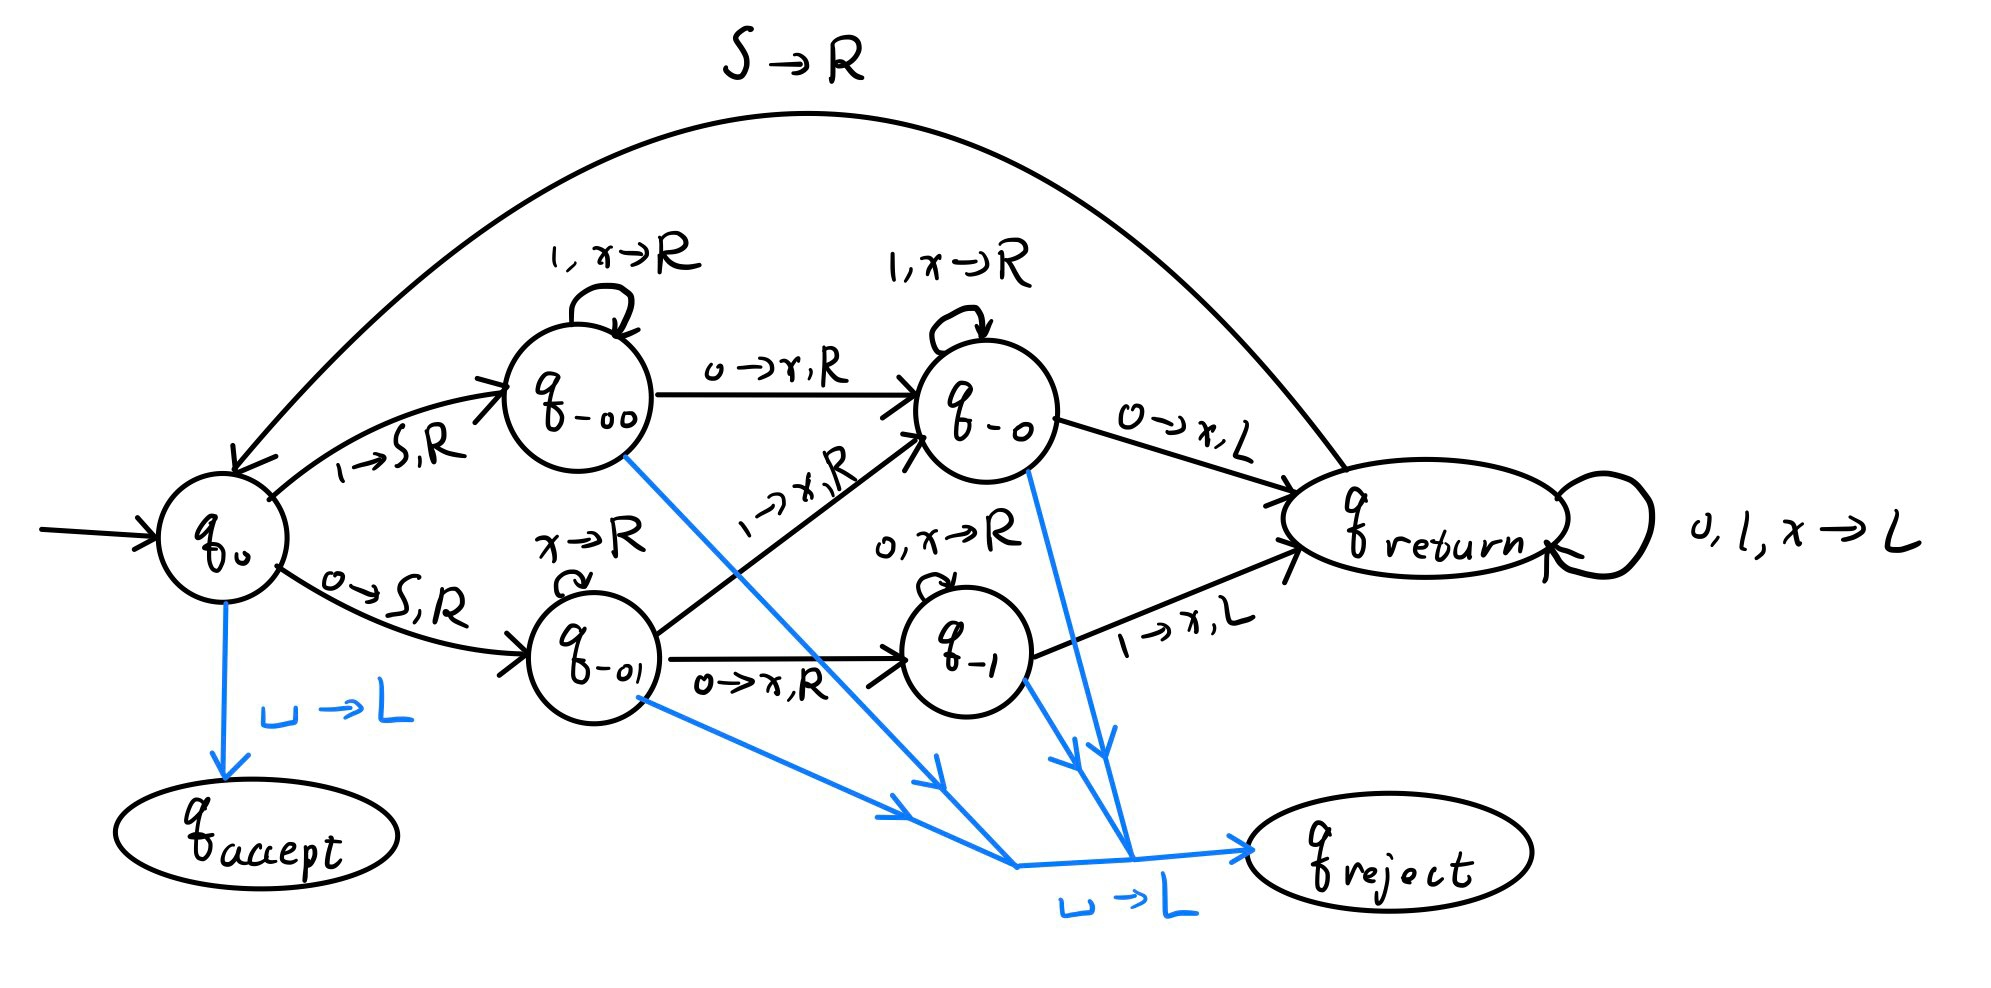
\includegraphics[width=10cm]{image/3.补充题2.png}
            \caption{3.补充题2}
            \label{fig:3_补充题2}
        \end{figure}

    \end{enumerate}
\end{solution}


\newpage


\problem{选做题:3.22} 设 $k$-PDA 表示有 $k$ 个栈的下推自动机. 因此,  $0$-PDA 就是一个NFA, $1$-PDA 就是通常的PDA. 已经知道$1$-PDA 比$0$-PDA 更强(识别更大的语言类). 
\begin{enumerate}
    \item 证明 $2$-PDA 比 $1$-PDA 更强. 
    \item 证明 $3$-PDA 不比 $2$-PDA 更强. 
\end{enumerate}

(提示:用两个栈来模拟一个图灵机带. )

\begin{proof}
    \begin{enumerate}
        \item 尝试用两个栈模拟一个图灵机带. 两个栈是相对的, 栈顶均存储对应图灵机读写头在纸带上的位置, 栈 (除了栈底标志\$外的) 最底部的一个字符为输入字符串两端的两个字符, 分别按顺序向中间压入所有字符串字符. 如果读写头的位置向右超出原本字符串的区域, 初次更改时表示右侧子串的栈会变空, 此时向左侧不断压栈即可, 这样能 ``延伸字符串长度''. (因为是选做题懒得写太仔细, 于是) 举个例子, 如图\ref{fig:3_22}, 为一个对应的例子.

        \begin{figure}[!htbp]
            \centering
            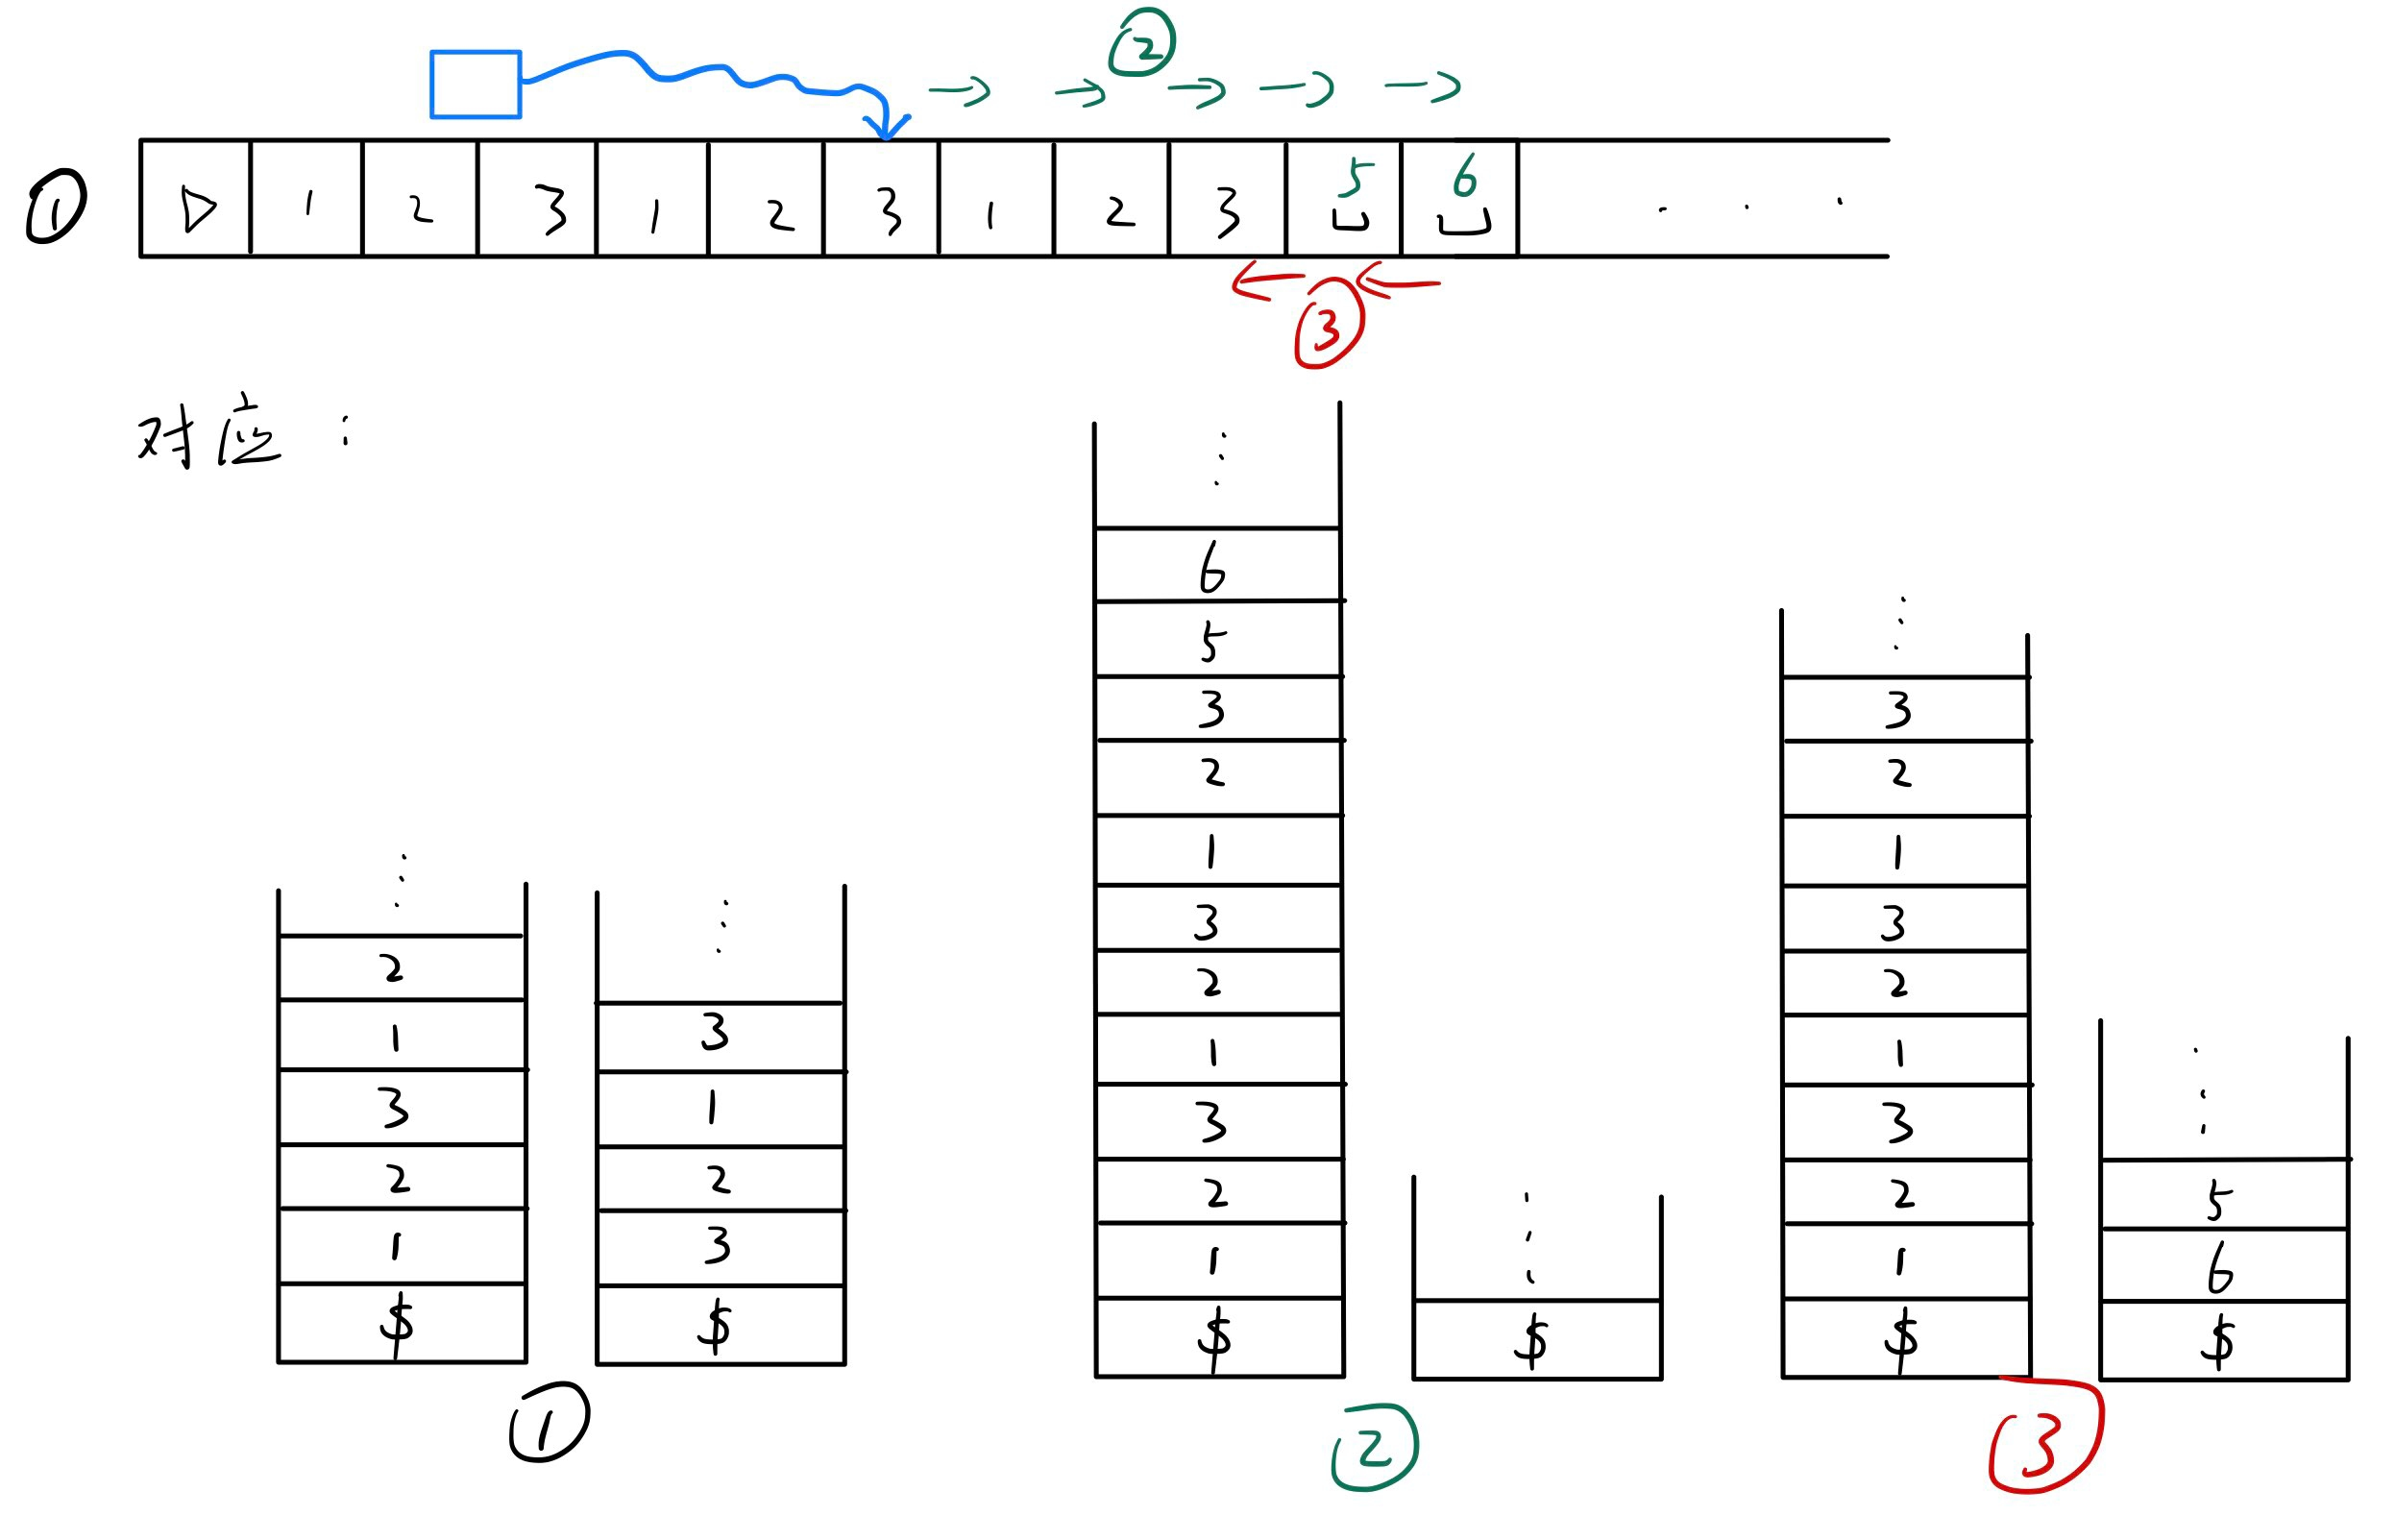
\includegraphics[width=10cm]{image/3.22.png}
            \caption{3.22}
            \label{fig:3_22}
        \end{figure}

        这样完全可以把纸带和两个栈等效起来.

        \item 一个很有意思的构造: 普通图灵机既然与两个栈等效, 那我们考虑与普通图灵机等效的另一类: 双无限带图灵机. 这类图灵机如果左半部分只用作一个栈 (很简单就可以做到这件事), 并且右半部分当作通用图灵机使用的话, 新产生的机器和$3$-PDA等效 (因为等效于三个栈), 表示能力不会比$2$-PDA更弱; 而其表示能力不会强过双无限带图灵机 (与普通图灵机等效, 进而与$2$-PDA等效), 因此不会比$2$-PDA更强. 
    \end{enumerate}
\end{proof}






\newpage


\textbf{第3.3次作业:3.15(b), 3.13}


\problem{3.15} 证明图灵可识别语言类在下列运算下封闭:

\problem{(b)} 连接

\begin{proof}
    对两个图灵可识别语言$A$, $B$, 分别构造对应的普通图灵机$M_A$, $M_B$能识别这两个语言. 构造一个有三带且可分别读写的图灵机. 规定三个纸带的功能如下:
    \begin{enumerate}
        \item 存放输入字符串, 并且只读不写.
        \item 可以存放从输入字符串中取出的一个子串, 并选择用普通图灵机$M_A$, $M_B$之一对之操作至多$n$次 ($n$为任意给定的正整数), 判断其是否已达到接受状态.
        \item 记录两个数据: 分割输入字符串为两个子串的位置; 将其操作的次数上限$n$.
    \end{enumerate}

    对这个新图灵机的作用描述: 对于正整数$n=1,2,3,\,\dots$, 依次增大$n$, 并进行如下操作:
    
    将输入字符串拆分成两个子串 (其连接为输入的字符串), 遍历每一种可能性, 分别对前串和后串模拟使用$M_A$, $M_B$进行至多$n$步的判定.
    
    如果两个字符串都获得模拟接受的结构, 那么接受输入字符串; 否则, 让$n$增大$1$, 循环进行这个操作.

\end{proof}


\problem{3.13} 证明:一个语言是可判定的, 当且仅当有枚举器以标准字符串顺序枚举这个语言. 

\begin{proof}
    ``$\Longrightarrow$'': 忽略输入. 对所有字符串按字典序排序, 依次投入枚举器中; 枚举器检查这个字符串是否在语言中 (由于这是个可判定的语言, 一定能进入停机状态, 不会无限运转而不停机), 如果进入接受格局, 则输出之, 否则不输出. 不断按顺序检查字符串, 枚举器会按字符串顺序给出任意一个语言中的字符串作为输出.

    ``$\Longleftarrow$'': 若 $L$ 是有限语言, 显然存在一个判定器 $M$ 识别 $L$: 其可用状态记录 $L$ 中的所有元素, 并将输入与记录的元素一一比对, 从而判定 $L$. 判定器显然会在有限步内停机.
    
    若 $L$ 是无穷语言, 判定器 $M$ 按如下方式运行 $M$ = "对于输入 $\omega$:
    \begin{enumerate}
        \item 运行 $E$, 每当 $E$ 输出一个串, 将其与 $\omega$ 比较
        \item 如果 $\omega$ 与该输出串相同, 则接受, 如果 $\omega$ 按字符串顺序排在该输出串之前, 则拒绝, 否则返回 1. 
    \end{enumerate}
    ". 由L 是无穷语言知, 其包含串 $\omega'$ 且 $\omega'$ 按字符串顺序排在 $\omega$ 之后. 枚举器 $E$ 将在有限步内枚举到 $\omega'$. 由于 $E$ 按照字符串顺序枚举, 因此枚举到 $\omega'$ 时便知 $\omega \notin L$.

    综上, $M$ 识别语言 $L$, 并在任意输入上都停机. 
\end{proof}




\end{document}
